\documentclass[letterpaper]{article}
\usepackage[utf8]{inputenc}
%\usepackage[ansinew]{inputenc}
\usepackage[spanish]{babel}
\usepackage{graphicx}

\begin{document}

\title{Anteproyecto 4\\ Laboratorio Control de Servomotores}
\author{
 Marco Antonio Montero Chavarría Carné: A94000\\
  \and
  Francisco Molina Carné: B14194\\  
}
\maketitle

\section{Investigación Previa}
\subsection{Servomotor}
 Un servomotor mejor conocido como servo es un dispositivo similar a un motor DC que tiene la capacidad de ubicarse en cualquier posición dentro de su rango de operación y mantenerse estable en dicha posición. Por lo tanto es un motor eléctrico al que se le puede controlar la posición.\\
 Esta conformado por un motor, una caja reductora y un circuito de control. En otras palabras un servo es un motor especial al que se le ha añadido un sistema de control, un potenciómetro y un conjunto de engranajes.\\
 Los servos hacen uso de la modulación por ancho de pulsos (PWM) para controlar la posición de los motores DC. La electrónica dentro del servomotor responderá al ancho de la señal modulada, por medio de un feedback de resistencia obtenida del potenciómetro y llevará el motor a la posición deseada.\\ Para el proyecto se utilizará alguno de los modelos TG69e, TYG-R5180MG o PARK HPX F. Todos modelos que permiten controlar posiciones entre 0º y 180º .
 \newpage
\subsection{PWM}
 La modulación por ancho de pulsos conocida como PWM, es una técnica en la que se modifica el ciclo de trabajo de una señal que sea periódica, ya sea para transmisión de información a través de un canal de comunicaciones o para controlar la cantidad de energía que se envía a una carga. Se tiene:\\
$D= \frac{ \tau }{T}$\\
Donde D es el ciclo de trabajo, $\tau$ es el tiempo en que la función es positiva y T es el período de la función.\\
La construcción típica de un circuito PWM se lleva a cabo mediante un comparador con dos entradas y una salida. Una de las entradas se conecta a un oscilador de onda de dientes de sierra, mientras que la otra queda disponible para la señal moduladora. En la salida la frecuencia es generalmente igual a la de la señal diente de sierra y el ciclo de trabajo está en función de la señal portador.
\subsection{PID}
 Un controlador PID es un mecanismo de control con una realimentación que se utiliza en control industrial o automático. Calcula la desviación o error entre un valor medido y un valor deseado.\\
 El algoritmo de control PID consta de tres parámetros importantes: el proporcional, el integral y el derivativo. El valor Proporcional depende del error actual. El integral depende de los errores pasados y el Derivativo es una predicción de los errores futuros. La suma de estos tres es usada para ajustar el proceso por medio de un elemento de control como la tensión en un calentador.\cite{1}\\

\begin{figure}[hbtp]
\centering
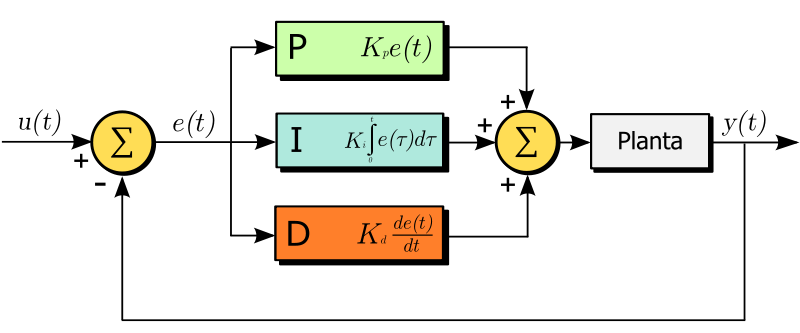
\includegraphics[width=10 cm]{PID.png}
\caption{Esquema PID}
\label{PID}
\end{figure}


\newpage
\section{Solución Propuesta}

Primero se ocupa un programa que controle los valores de velocidad y posición que se envían al servomotor, ya que estos servomotores no cuentan con un feedback de la posición se debe tomar el motor como una planta conocida y elaborar un controlador de velocidad para llegar con la velocidad deseada a la posición requerida. Esto se puede lograr con un programa en python que escriba en los pines de salida que se definan para controlar el servomotor con el programa realizado en C, es muy parecido al programa que se utilizó en el proyecto 3 que lee los pines PA0,PA1,PA2; con la adición en el programa de un método que escriba en los pines y modifique los valores del PWM de salida para que se ajuste la posición con la velocidad que se busca en el servo.\\
Esto se puede lograr con la librería usada en el proyecto anterior -pyserial- ya que tiene opciones de envio al puerto designado para comunicación serial. Por lo tanto por el micro-usb se comunicará el programa del usuario que ingresa el dato de velocidad y posición y genera un control pid que envía pulsos en pwm al programa en C flasheado en el -stm32f4-.\\
Naturalmente para evitar conflicto entre ambas comunicaciones se necesitará correcto uso de los métodos para cerrar y abrir la comunicación entre el microcontrolador y el computador que se este utilizando para enviar los valores.\\
Por último con la librería matplotlib se pueden tomar los valores de un pin extra conectado a un potenciómetro o algún otro sensor para recibir del microcontrolador y gráficarlos contra el tiempo para observar su variación.\\

\begin{center}
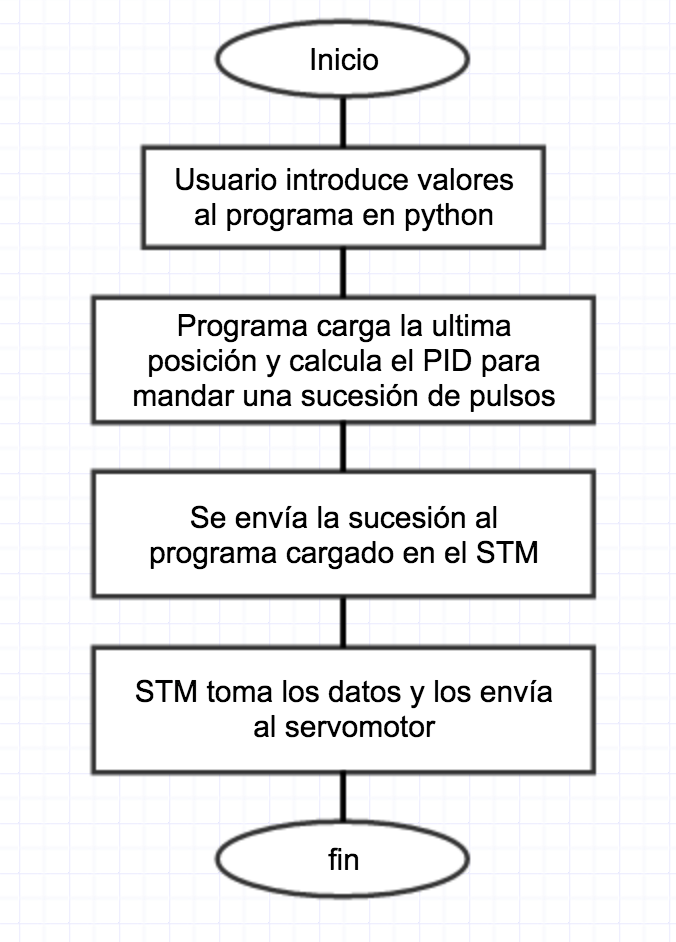
\includegraphics[width=6cm]{micro.png}
\end{center}

El otro problema del proyecto es la parte física electrónica, ya que el PWM con el que se debe manipular la velocidad y posición del servomotor, necesita valores entre 0 y 5V y lo máximo que se puede obtener directamente del -stm- es 0-3V por lo tanto se debe utilizar un amplificador operacional en configuración de amplificador no inversor con alimentación de 5V, esto para llegar a obtener el rango deseado para el PWM. Una configuración como esta luce de la siguiente forma:\\

\begin{center}
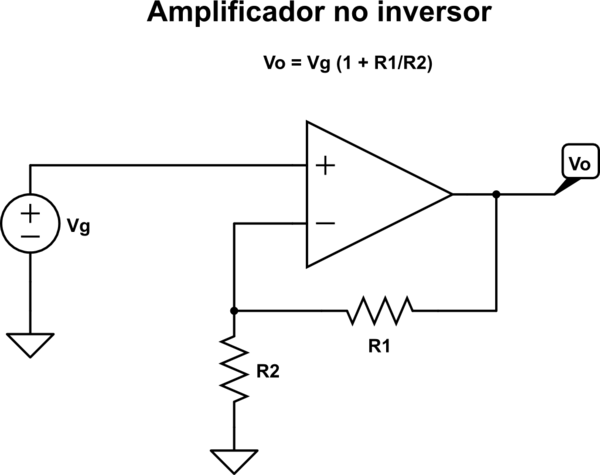
\includegraphics[width=5cm]{amp.png}
\end{center}

Los valores de las resistencias se ajustarán según el valor real que se tenga en el laboratorio para obtener el rango deseado en la salida de la configuración no inversor.\\

Básicamente se buscará crear un sistema de control con un lazo de realimentación donde la señal realimentada será el PWM, esta señal dará por lo tanto una estimación de cual es el estado del servomotor, ya que por su diseño, el mismo no puede brindar esa información al stm32f4. Y a partir de esa señal PWM se buscará modificarla lo necesario para alcanzar un nuevo valor en las variables controlodas, que en el caso de este proyecto serán la velocidad y la posición, como se han mencionado exhaustivamente.

\section{Procedimiento}
\begin{itemize}
\item Crear el código en python para comunicación serial y graficación.
\item Crear el código en c que tome los datos enviados por comunicación serial y que envié el PWM y tome datos de salida del servo.
\item Crear el circuito físico del amplificador operacional no inversor para lograr el rango de PWM deseado.
\end{itemize}

\section{Observaciones y recomendaciones}

\begin{itemize}
\item Tener sumo cuidado con el circuito de protección, probar que las tensiones sean las adecuadas.
\item Realizar pequeñas pruebas antes de programar cada parte y descomponer el problema en problemas más sencillos.
\item Probar el circuito de amplificación por fuera con un generador de señales para no quemar el STM32f4 por un pico de tensión en caso de un error en el diseño de la configuración amplificadora.
\end{itemize}

\bibliographystyle{alpha} 
\bibliography{refs}



\end{document}
